\section*{Resolução da Questão 2: Busca Gulosa e A*}

\subsection*{A) Estruturação Lógica do Problema}

A formulação heurística do robô em malha com bloqueios:

\begin{itemize}
    \item \textbf{Formato de Estado}: Cada localização mapeada no piso é definida por um símbolo. Exemplo: $s \in \{A, B, C, \dots, T\}$.
    \item \textbf{Início}: A partida ocorre na célula $A$.
    \item \textbf{Encerramento}: Chega-se ao fim se e somente se $s = T$.
    \item \textbf{Regras de Transição}: Vizinhos disponíveis e seus pedágios de travessia. Por exemplo: $Vizinhos(A) = \{(B, 2), (C, 4), (D, 3)\}$.
    \item \textbf{Cálculo de Custos ($g$)}: O valor $g(n)$ rastreia o peso acumulado de todas as rotas percorridas desde o nó base $A$ até o destino local $n$.
    \item \textbf{Impacto da Heurística ($h$)}: Representação de um "palpite instruído" do esforço restante de $n$ até $T$. No A*, a subestimação estrita do verdadeiro custo ($h(n) \le h^*(n)$) confere à heurística o status de "admissível", travando a rota como matematicamente perfeita (ótima).
\end{itemize}

\subsection*{B) Avaliação com Greedy Best-First Search}

A tática gulosa guia as decisões avaliando cegamente $f(n) = h(n)$, ignorando pedágios já pagos.

\textbf{Desempenho (Greedy):}
\begin{itemize}
    \item \textbf{Trilha Encontrada:} A $\rightarrow$ C $\rightarrow$ H $\rightarrow$ O $\rightarrow$ T
    \item \textbf{Custo Acumulado:} 19
    \item \textbf{Quantia de Nós Expandidos:} 5
    \item \textbf{Quantia de Nós Gerados:} 9
\end{itemize}

\textbf{Passo-a-Passo Guloso:}
\begin{table}[h!]
\centering
\small
\begin{tabular}{|c|c|c|l|}
\hline
\textbf{Turno} & \textbf{Expansão} & \textbf{$h(n)$} & \textbf{Fila Prioritária por $h$} \\ \hline
1 & A & 10 & [C(7), B(8), D(9)] \\ \hline
2 & C & 7 & [H(4), G(6), B(8), D(9)] \\ \hline
3 & H & 4 & [O(1), N(4), G(6), B(8), D(9)] \\ \hline
4 & O & 1 & [T(0), N(4), G(6), B(8), D(9)] \\ \hline
5 & T & 0 & Concluído com sucesso \\ \hline
\end{tabular}
\end{table}

\textbf{Árvore de Exploração Parcial (Greedy):}
\textit{Preenchimento roxo (\textcolor{purple}{Cor}) para explorados. Verde (\textcolor{teal}{Cor}) para o nó final.}

\begin{center}
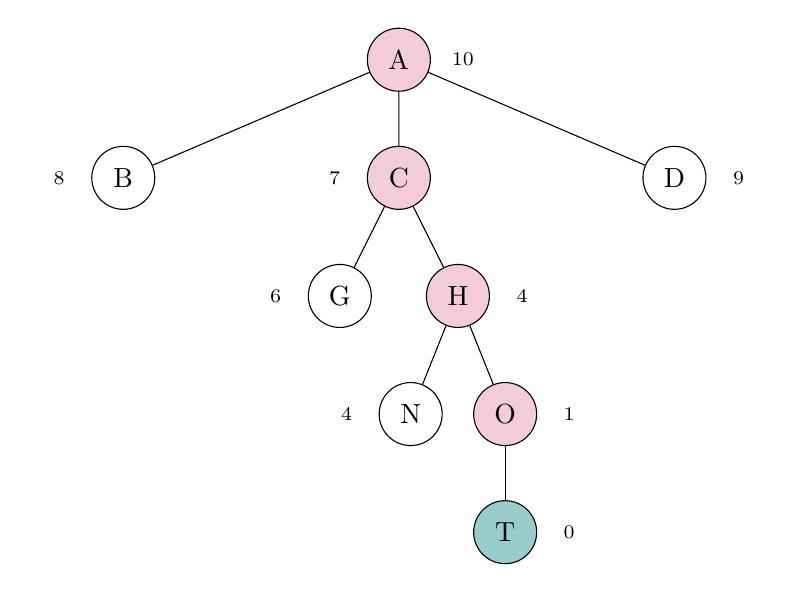
\begin{tikzpicture}[level distance=1.5cm,
  level 1/.style={sibling distance=3.5cm},
  level 2/.style={sibling distance=1.5cm},
  level 3/.style={sibling distance=1.2cm},
  every node/.style={circle, draw, minimum size=0.8cm, inner sep=1pt}]
  
  \node[fill=purple!20, label=right:{\scriptsize 10}] {A}
    child {node[label=left:{\scriptsize 8}] {B}}
    child {node[fill=purple!20, label=left:{\scriptsize 7}] {C}
        child {node[label=left:{\scriptsize 6}] {G}}
        child {node[fill=purple!20, label=right:{\scriptsize 4}] {H}
            child {node[label=left:{\scriptsize 4}] {N}}
            child {node[fill=purple!20, label=right:{\scriptsize 1}] {O}
                child {node[fill=teal!40, label=right:{\scriptsize 0}] {T}}
            }
        }
    }
    child {node[label=right:{\scriptsize 9}] {D}};
\end{tikzpicture}
\end{center}

\newpage
\subsection*{C) Avaliação com Algoritmo A*}

A* equilibra os pesos do passado e previsões futuras: $f(n) = g(n) + h(n)$.

\textbf{Desempenho (A*):}
\begin{itemize}
    \item \textbf{Trilha Encontrada:} A $\rightarrow$ B $\rightarrow$ F $\rightarrow$ K $\rightarrow$ R $\rightarrow$ T
    \item \textbf{Custo Acumulado:} 17
    \item \textbf{Quantia de Nós Expandidos:} 20
\end{itemize}

\textbf{Passo-a-Passo A*:}
\begin{table}[h!]
\centering
\scriptsize
\begin{tabular}{|c|c|c|c|c|l|l|}
\hline
\textbf{Trn} & \textbf{Nó} & \textbf{$g$} & \textbf{$h$} & \textbf{$f$} & \textbf{Fila (Nó:f)} & \textbf{Rota} \\ \hline
1 & A & 0 & 10 & 10 & [B:10, C:11, D:12] & A \\ \hline
2 & B & 2 & 8 & 10 & [C:11, E:11, D:12, F:12] & A-B \\ \hline
3 & C & 4 & 7 & 11 & [E:11, D:12, F:12, G:14, H:14] & A-C \\ \hline
4 & E & 5 & 6 & 11 & [D:12, F:12, G:14, H:14, J:14] & A-B-E \\ \hline
5 & D & 3 & 9 & 12 & [F:12, I:12, G:14, H:14, J:14] & A-D \\ \hline
6 & F & 7 & 5 & 12 & [I:12, K:13, G:14, H:14, J:14, L:18] & A-B-F \\ \hline
7 & I & 5 & 7 & 12 & [K:13, G:14, H:14, J:14, L:18, P:18] & A-D-I \\ \hline
8 & K & 10 & 3 & 13 & [G:14, H:14, J:14, R:15, L:18, P:18] & A-B-F-K \\ \hline
9 & G & 8 & 6 & 14 & [H:14, J:14, R:15, M:17, L:18, P:18] & A-C-G \\ \hline
10 & H & 10 & 4 & 14 & [J:14, O:15, R:15, M:17, N:17, L:18, P:18] & A-C-H \\ \hline
11 & J & 9 & 5 & 14 & [O:15, R:15, M:17, N:17, Q:17, L:18, P:18] & A-B-E-J \\ \hline
12 & O & 14 & 1 & 15 & [R:15, M:17, N:17, Q:17, L:18, P:18, T:19] & A-C-H-O \\ \hline
13 & R & 13 & 2 & 15 & [M:17, N:17, Q:17, T:17, L:18, P:18] & A-B-F-K-R \\ \hline
14 & M & 14 & 3 & 17 & [N:17, Q:17, S:17, T:17, L:18, P:18] & A-C-G-M \\ \hline
15 & N & 13 & 4 & 17 & [Q:17, S:17, T:17, L:18, P:18] & A-C-H-N \\ \hline
16 & Q & 13 & 4 & 17 & [S:17, T:17, L:18, P:18] & A-B-E-J-Q \\ \hline
17 & S & 16 & 1 & 17 & [T:17, L:18, P:18] & A-C-G-M-S \\ \hline
18 & L & 12 & 6 & 18 & [T:17, P:18] & A-B-F-L \\ \hline
19 & P & 10 & 8 & 18 & [T:17] & A-D-I-P \\ \hline
20 & T & 17 & 0 & 17 & Sucesso & A-B-F-K-R-T \\ \hline
\end{tabular}
\end{table}

\textbf{Árvore de Exploração Parcial (A*):}
\textit{Legenda: Expansões em roxo (\textcolor{purple}{Cor}). Trilha perfeita em negrito com tom verde-escuro.}

\begin{center}
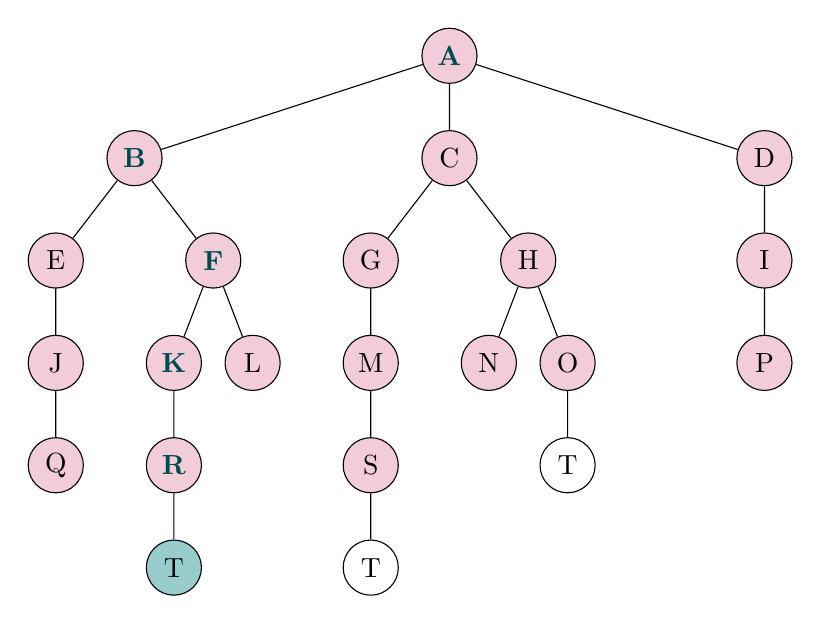
\begin{tikzpicture}[level distance=1.3cm,
  level 1/.style={sibling distance=4cm},
  level 2/.style={sibling distance=2cm},
  level 3/.style={sibling distance=1cm},
  every node/.style={circle, draw, minimum size=0.7cm, inner sep=1pt}]
  
  \node[fill=purple!20, font=\bfseries\color{teal!60!black}] {A}
    child {node[fill=purple!20, font=\bfseries\color{teal!60!black}] {B}
      child {node[fill=purple!20] {E} child {node[fill=purple!20] {J} child {node[fill=purple!20] {Q}}}}
      child {node[fill=purple!20, font=\bfseries\color{teal!60!black}] {F} 
        child {node[fill=purple!20, font=\bfseries\color{teal!60!black}] {K} child {node[fill=purple!20, font=\bfseries\color{teal!60!black}] {R} child {node[fill=teal!40] {T}}}}
        child {node[fill=purple!20] {L}}
      }
    }
    child {node[fill=purple!20] {C}
      child {node[fill=purple!20] {G} child {node[fill=purple!20] {M} child {node[fill=purple!20] {S} child {node {T}}}}}
      child {node[fill=purple!20] {H} child {node[fill=purple!20] {N}} child {node[fill=purple!20] {O} child {node {T}}}}
    }
    child {node[fill=purple!20] {D}
      child {node[fill=purple!20] {I} child {node[fill=purple!20] {P}}}
    };
\end{tikzpicture}
\end{center}

\subsection*{D) Experimento: Distorção das Heurísticas}

Injetamos erros nos sensores de estimativa:
\begin{itemize}
    \item $h(D)$ alterado para $2$
    \item $h(I)$ alterado para $1$
    \item $h(B)$ alterado de 8 para $22$
\end{itemize}

\textbf{Comparativo do Impacto:}
\begin{table}[h!]
\centering
\begin{tabular}{|l|l|c|c|}
\hline
\textbf{Abordagem} & \textbf{Rota Consolidada} & \textbf{Preço} & \textbf{Expansões} \\ \hline
Guloso (Padrão) & A $\rightarrow$ C $\rightarrow$ H $\rightarrow$ O $\rightarrow$ T & 19 & 5 \\ \hline
Guloso (Corrompido) & A $\rightarrow$ C $\rightarrow$ H $\rightarrow$ O $\rightarrow$ T & 19 & 7 \\ \hline
A* (Padrão) & A $\rightarrow$ B $\rightarrow$ F $\rightarrow$ K $\rightarrow$ R $\rightarrow$ T & 17 & 20 \\ \hline
A* (Corrompido) & A $\rightarrow$ C $\rightarrow$ H $\rightarrow$ O $\rightarrow$ T & 19 & 13 \\ \hline
\end{tabular}
\end{table}

\textbf{Síntese dos Efeitos:}
\begin{enumerate}[label=\roman*)]
    \item A rota A* degenerou, abandonando o caminho ideal (17) por um sub-ótimo (19).
    \item A causa direta da falha do A* reside no fato de $h(B)=22$ ser uma superestimativa extrema, violando a prova matemática de admissibilidade do A*.
    \item A pesquisa Gulosa reagiu vagamente nos fundos falsos (testou D primeiro pois $h=2$), mas em geral re-encontrou a mesma trilha sub-ótima sem maiores prejuízos lógicos.
\end{enumerate}

\subsection*{E) Conclusões Gerais}

O A* é incontestável como líder em confiabilidade para malhas difíceis. Enquanto a busca gulosa desce rapidamente rampa abaixo (frequentemente trombando em obstáculos e achando percursos longos em forma de $U$), o A* se resguarda conferindo $g(n)$, e é o único blindado com garantias matemáticas de otimalidade na literatura, condicionada à pureza de seu estimador heurístico $h(n)$.
